%% UTF-8
\documentclass[twoside, workbib, UTF8, phd]{nputhesis}
\usepackage[backend=biber,
            style=gb7714-2015,
            doi=false]{biblatex}
\addbibresource{ref.bib}        % biblatex 命令. 添加参考文献文件, 必须加后缀.

\schoolno{10699}
\classno{O.242}
\secretlevel{公开}
\authorno{2018999999}

\title[\LaTeX\ Template for Thesis of NPU]{西北工业大学硕博士论文\LaTeX 模板}

\author[San Zhang]{张\,\,三}
\major[Mathematics]{数学}
\supervisor[Si Li]{李四}
\applydate[April 2018]{2018~年~4~月}
\support{本文研究得到某某基金(编号:XXXXXXX)资助。}

\begin{document}
\makecover    % 生成中英文封面.
\frontmatter  % 分割封面与前言部分.

% 中文摘要
\begin{abstract}
  本模板基本实现了官方格式要求: 封皮, 页眉页脚, 章节标题格式, 参考文献格式等.
  \begin{keywords}
    论文模板,西工大
  \end{keywords}
\end{abstract}

% 英文摘要
\begin{Abstract}
   some meaningless words.
  \begin{Keywords}
    Thesis Template, NPU
  \end{Keywords}
\end{Abstract}

\tableofcontents    % 目录
\printnomenclature  % 符号命名表 添加符号可用 \nomenclature{<sym>}{<text explanation>}
\mainmatter         % 分割目录和正文部分

\chapter{本模板内容}

\section{包含内容}
原版来自https://github.com/lrtfm/nputhesis,可以自行下载原版,不想看我的这个版本的话。\par\par
包含的内容见下图,如有多余。。。
% 图片示例
\begin{figure}[htbp]
    \centering
    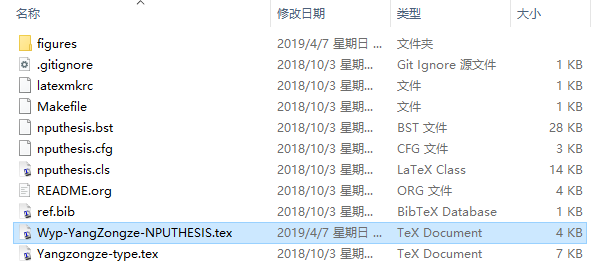
\includegraphics[width=0.8\textwidth]{figures/fig-files.png}
    \caption{包含的文件}
\end{figure}

\section{编译中会产生的文件}
编译过程中会产生很多中间文件,如有疑问的,建议删掉\par
可以删掉的文件见下表所示:
% 表格示例 三线表
\begin{table}[htbp]
  \caption{可以删掉的文件}
  \centering
  \begin{tabular}{lccccccccc}
    \toprule
     可删文件 & .& .& .& .& .& .& .& .& . \\
    \midrule
    扩展名 &bbl&gz&xml&blg&pdf&out&log&aux&bcf\\
    \bottomrule
  \end{tabular}
\end{table}

\chapter{本模板使用方法}
编译方法及运行。。。
\section{成功方案}
先安装Miktex,大概200M,不大。\par
然后cmd 输入mpm 进入packages 全装了吧,西工大网速还可以,二十分钟差不多。。。
\section{编译方法}
点击NPUTHESIS-Yzz-Wyp.tex文件(NPUTHESIS-Yzz-type.tex是原版模板貌似Yangzongze大佬作品,本人斗胆略作修改和说明),texworks打开,左上角选择编译方法\par
先Xelatex\par\par
再Biber\par\par
再Xelatex\par\par
保险起见,再来一次Xelatex。
之后如果修改了结构,需要连续两次Xelatex,毕竟要生成目录索引的。


\chapter{参考文献事宜及模板缺陷}
建议使用谷歌学术,搜索之后点cite,点bicite,然后出来个网页,全选,复制,粘贴到.bib文件中,如\par
学习可以参考文献\cite{Knuth1986,Lamport1994,Liu2013}, 其中 \cite{Liu2013} 最适合入门.参考文献用的GB/T 7714-2015,应该没问题。
\section{存在的问题}
外封面不对。。。\par
前辈 Zongze Yang 估计嫌费劲吧,我是不会改。。。\par
不过没关系感觉,毕竟打印的时候不用外封面。不会改也不用纠结。。\par\par
另,空白页不是错误。学校要求章节第一页必须在单面页的。

\backmatter
% 参考文件章
\printbibliography     % biblatex 输出参考文件方式
%附录
\Appendix  % 如果有多个附录, 可重复使用该命令, 自动按字母编号.
% 致谢
\Thanks 
\Work
%  biblatex 方式 \papersection{<bib-key-list>}
% \papersection{Knuth1986}
%  multibib 方式 \papersection[<bibstyle>]{<bib-file>}{<bib-key-list>}
% \papersection[nputhesis]{ref}{Knuth1986}
%  none  方式 即手动书写方式
\papersection  % 以下填写发表论文情况
1. 论文1
\researchsection % 以下填写参加科研情况
1. 我的研究项目1
\statement
\end{document}
